\section{Recrossing Effect}
\label{sec:recrossing}
%focus, schwerpunkt, emphasis

%In the last section, we have seen that the projected transfer operator of a Markov process respectively its matrix representation inherit some of the most important properties of the original process. Two further desirable properties would be the maintainance of Markovianity and a correct long-time description of the Markov State Model. We will examine these two issues in this section
%For instance, one further desirable property would be a commuting behaviour in/concerning propagation and projection of the process. That is, it should make no difference in which order these two operations are executed.
%That is, it should make no difference if we propagate a projected process or if we project a propagated %process.
%Unfortunately/but it will turn out that this is not the case.

%examine/introduce. crucial/main points/issues/subjects/topics of this thesis. This effect, occuring/appearing
In this section, we are going to examine the so called \textit{Recrossing Effect} which is one of the main topics of this thesis.
\marginpar{relation to iteration error}
%arising
This effect, occuring when projecting a process onto a smaller state space, may spoil the Markov Property of the process. \marginpar{measure by $S$?}
\marginpar{kind of memory effect}

We are going to analyze it by means of an easy example.
%with the help of an easy example.
Additionally, we have to face the problem that a projected process/transfer operator does not necessarily behaves/propagates as the original process. We will explain the relevance of this \textit{iteration error} without going into further details, since in the following chapters we will be able to apply a projection where this error/deviation vanishes.
%not in all chapters ;) only \ref{sec:rebinding}
%without going into further/deeper details/focus/emphasis,
%perform/execute/apply

%Furthermore, we will see the relation between the matrix representation from theorem \ref{thm:galerkin} %on the rebinding effect and how this effect can be measured considering the matrices $S$ and $T$.
%We will also compute some error estimations/bounds for the recrossing effect.

%In MD, the recrossing effect is also called \textit{rebinding effect}. Since the examination of the rebinding %effect is one of the main objectives of this thesis, we will put much emphasis on the mathematical %description of this effect.

%Now what is the stochastic interpretation of theorem \ref{thm:galerkin}? Can we get some insight into the %nature of $G \Pcal G$? $T$ is a transition matrix? Its Markovianity is spoiled by $S$? The closer $S$ is to the %unit matrix, the smaller the Recrossing effect?
%It will be examined later in section 2.4 after we examined the so called Recrossing effect which describes %the loss of Markovianity by projecting the process/ transfer operator. By $S$ and $T$, the recrossing effect %can be measured.

\subsubsection*{Initial Situation}

Assume we are given a Markov process $(X_t)_{t \in \T}$ on a continuous or very large state space $\X$, described by the transfer operator $\Pcal := \Pcal(\tau)$.
% discretize the time
In order to get a discrete process out of it, we are going to project the time onto $\mathbb{N}$ and the state space onto a finite set $\{1,\dots,n\}$.
%is easy/naturally
Discretizing the time can be done naturally without problems since for every lag-time $\tau > 0$, the process $(X_{k\tau})_{k\in \mathbb{N}}$ is again Markovian. \marginpar{why?}

%examined/observed
However, the state-space discretization has to be observed a bit more elaborated.
Let's do this on the example of a full partition discretization.

%Assume we have fixed a lag-time $\tau > 0$ and are given the transfer operator $\Pcal := \Pcal(\tau)$ of a Markov process $(X_t)_{t \in \T}$.

%project if afterwards
%If we first propagate the process and then project it.
% the (original) process
Consider the operator $G(\Pcal^k) := G\Pcal^k G$, that is we first propagate the process and project it afterwards. Then for all $k$-multiples of $\tau$, we assign the current state of the original process $X_t$ to the projected process $\widetilde{X}_k$:
\begin{equation*}
\widetilde{X}_k = i \Leftrightarrow X_{k\tau} \in A_i.
\end{equation*}
The process $\xtilde_k$ describes the \textit{snapshot dynamics} of $X_t$ with lag time $\tau$ between the partition sets $A_1,\dots,A_n$.
The so defined process is not necessarily Markovian, since $(G(\Pcal^k))_k$ is in general \textbf{not} a semigroup. \marginpar{see ..}

\subsubsection*{Rebinding in a Double Well Potential}

%describing ... the motion of a particle?... in a double-well potential
Let $X_t$ be the Markov process corresponding to the double-well potential $V(x) = (x^2-1)^2$. We consider a full-partition of the state space into two sets $A$ and $B$ around the local minima of the energy landscape, as shown in figure \ref{fig:doublewell}.
\begin{figure}[!ht]
	\centering
	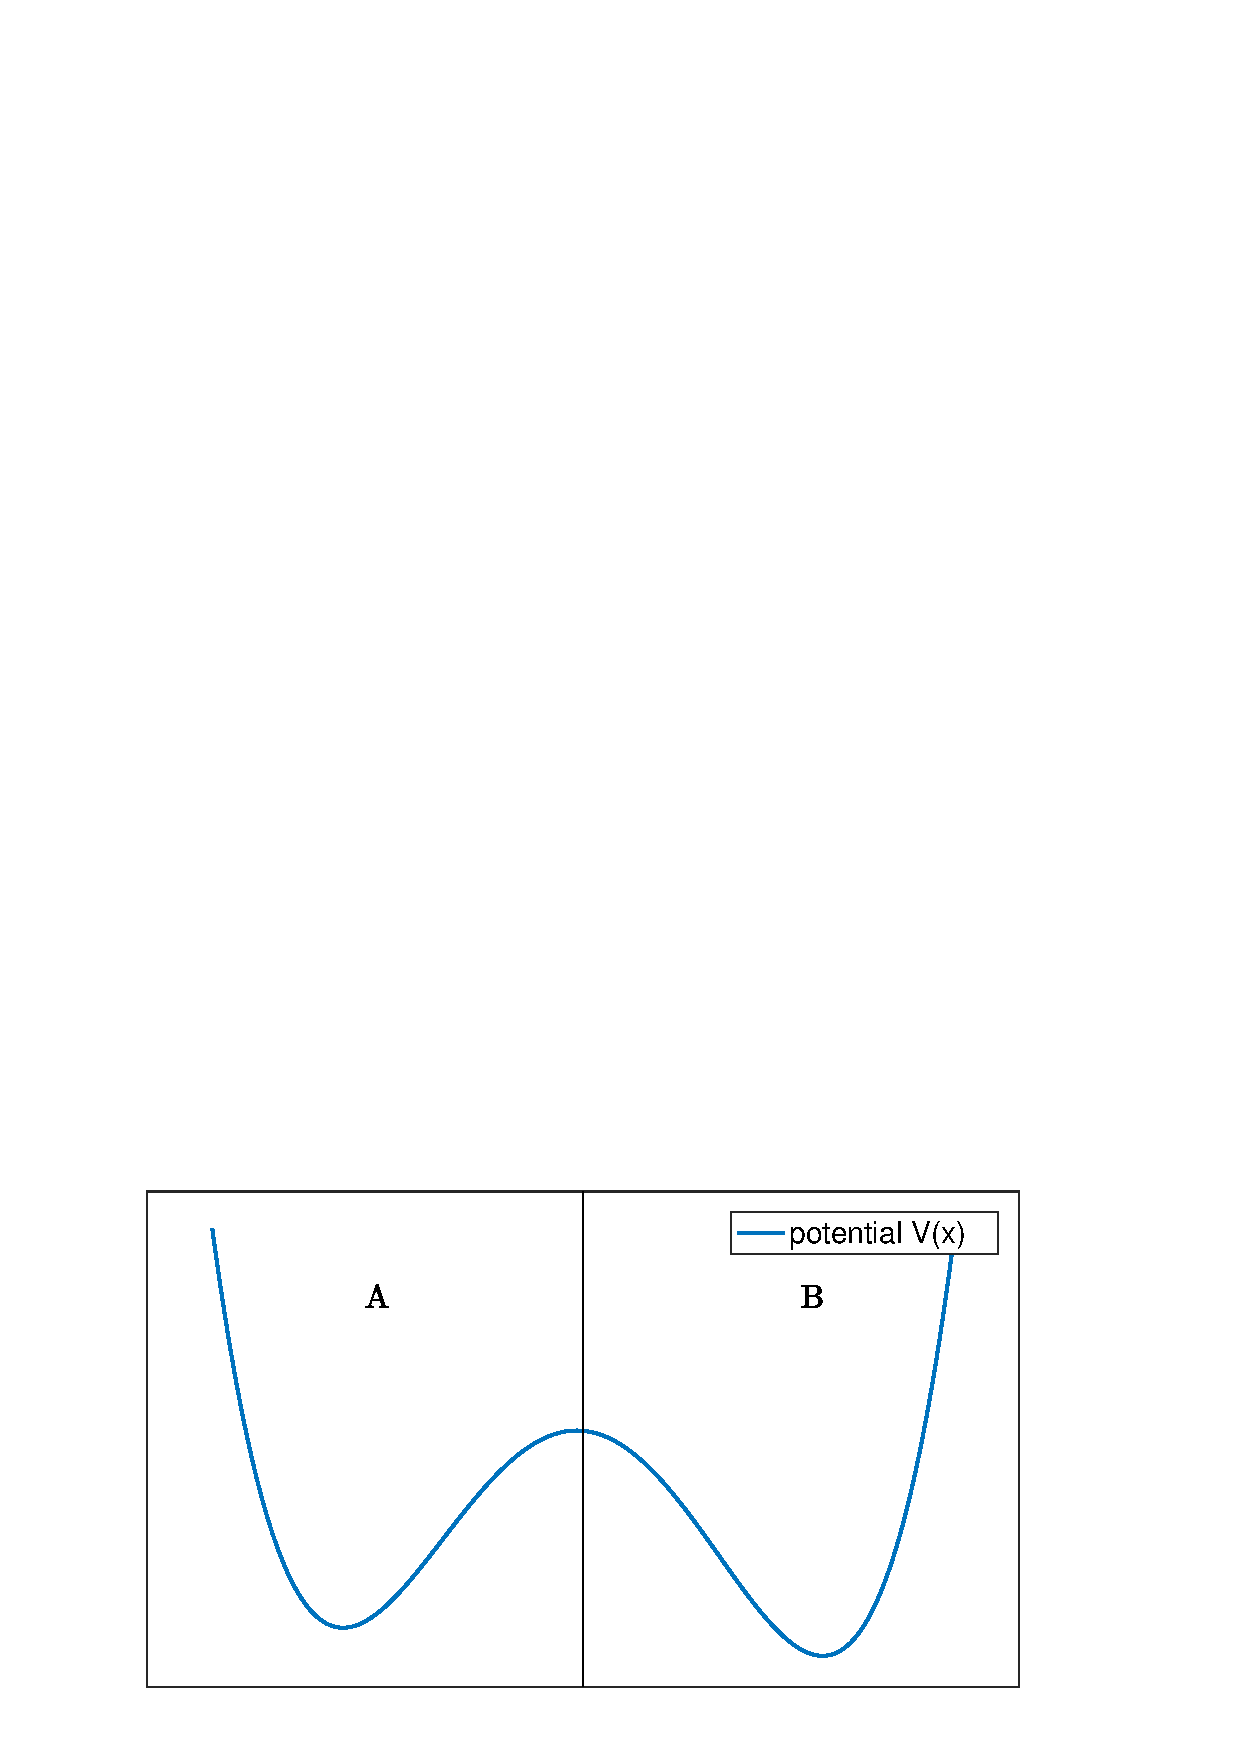
\includegraphics[width=0.6\textwidth]{Python/doublewell.png} %70% der Textbreite
	\caption{Full-partition of a double-well potential}
	\label{fig:doublewell}
\end{figure}
We are interested if the induced process $\xtilde_k$ inherits the Markovianity of $X_t$ or if it contains any memory effects.
%contains/includes

For a small lag-time $\tau = 0.1$ we compute the probability of $\xtilde_k$ to make a transition from $B$ to $A$ in one time-step. We compare it to the probability of the same transition with the \textbf{additional} information of having been in $B$ one time-step before/earlier. If the process was Markovian, then this additional information about the past should make no difference and thus, both probabilities should be equal.
We compute them in terms of the original process $X_t$ by
\begin{equation*}
\Prob_\mu[X_{(k+1)\tau} \in A \mid X_{k\tau} \in B] \textrm{ and }
\Prob_\mu[X_{(k+1)\tau} \in A \mid X_{k\tau} \in B, X_{(k-1)\tau} \in A].
\end{equation*}
Using the density functions $v_B$ and $v_{BA}$, we get \marginpar{$v$ densities?}
\begin{equation}
\label{eq:recrossing1}
\Prob_\mu[X_{(k+1)\tau} \in A \mid X_{k\tau} \in B] = \int_A v_B^\tau(x) \diff x = ... ,
\end{equation}
\begin{equation}
\label{eq:recrossing2}
\Prob_\mu[X_{(k+1)\tau} \in A \mid X_{k\tau} \in B, X_{(k-1)\tau} \in A] = \int_A v_{BA}^\tau(x) \diff x = ... .
\end{equation}
So we see that for such a short lag-time $\tau$, the process $\xtilde_k$ is \textbf{not} independent of the past  and hence \textbf{not} a Markov process.
%the process $\xtilde_k$ is \textbf{not} memoryless
%That behaviour is intuitively clear.
Equation \eqref{eq:recrossing1} describes the probability to get from $B$ to $A$, where ``being in $B$'' could mean everything from ``close to the transition region'' to ``far away from the transition region''. So this probability is averaged over \textbf{all} possible starting points in $B$. \marginpar{?}
We compare it to \eqref{eq:recrossing2}, where being in $A$ shortly before
%immediately one time-step; moving to B
being in $B$ increases the probability to return/recross to $A$ again.
This behaviour can be interpreted such that for a short time after a \textbf{transition}, the process is likely to be still inside ot the \textbf{transition region}.
In our example, the transition region is the area/region close to the maximum of potential energy. Thus, there is still an increased probability to return to the previous state.
%not only for this example true

%transition between states = crossing the ``barrier'' between the states..

%the probability that the process is still in the transition region. And to get to $A$ from the transition region in $B$ is just more likely than from any other region inside $B$.
%favorable spatial situation?

This issue is called the \textit{recrossing effect}, since additional memory \marginpar{recross the barrier?}
%as in \eqref{eq:recrossing2}
leads to an increased probability to ``recross'' shortly after a transition.
%when still being inside a transition region.
On the other hand, if we choose a large lag-time $\tau = 100$, then the past transition from $A$ to $B$ in \eqref{eq:recrossing2} took place a long time ago. So we cannot certainly know if the process is still in the critical transition region; during that long lag-time it could also have been gone anywhere else.
%That means that we could describe the memory effect of $\xtilde$ as a \textit{short-time memory}.
That means that the memory effect included in $\xtilde_k$ becomes smaller for larger lag-times and thus can be considered as a \textit{short-time memory}.

\subsubsection*{Comparison to Markov State Model}

After having observed the \textit{recrossing effect} as a memory effect when projecting the time-series(?) of a given continuous process onto a finite subspace, we want to compare that result to the corresponding \textit{Markov State Model}. \marginpar{def MSM}

So far, we considered the process $\xtilde_k$ belonging to the operator $G(\Pcal^k)$.
%Now, we want to consider the Markov State Model, i.e. the process $\xhat_k$ which is described by the operator $(G(\Pcal))^k$. The corresponding matrix representation is given by $P_c$ (see theorem \ref{thm:galerkin}).
Now, let $(\widehat{X}_k)_{k\in\mathbb{N}}$ be the Markov chain that is described by the transition matrix $P_c$, i.e. the matrix representation of the discretized transfer operator $G(\Pcal) := G\Pcal G$.
\\

A desirable behaviour of this model would be that $\widehat{X}_k$ and $\widetilde{X}_k$ have the same trajectory when started on the same initial distributions $\widehat{X}_0$ and $\widetilde{X}_0$. It will turn out that this is normally not the case.
%Another desirable property would be Markovianity of both models, since this is the case for the original process $X_t$. But we have alredy seen in theorem \ref{thm:galerkin} that the matrix representation $P_c$ of $G\Pcal G$ is in general not a transition matrix, i.e. $\widehat{X}_k$ is not Markovian
%shown/visualized
This question is visualized in diagram \ref{fig:diagram_transfer}.
Does it make a difference if we first project the process and then propagate it and vice versa?

\begin{figure}[!ht]
	\centering
	\begin{tikzcd}
	&  \Pcal(\tau) \arrow{d}{proj.} \arrow{r}{\tau \rightarrow \tau k}    & (\Pcal(\tau))^k \arrow{d}{proj.} 			\\
	G(\Pcal(\tau)) \widehat{=} &  P_c (\tau)   \arrow{r}{\tau \rightarrow \tau k}            &  (P_c(\tau))^k \\
\end{tikzcd}
\caption{Projecting/propagating a transfer operator (non-commutative)}
\label{fig:diagram_transfer}
\end{figure}
%\ref{fig:diagram_transfer}
%Weber shows in habilitation that under a certain Galerkin Projection using membership functions (not    %set-based family) leads to a commuting diagram of projection and propagation. \marginpar{non-reversible?}
%+ Markov Property is preserved? \marginpar{due to proj. or trans.op.?}
In general, this diagram is \textbf{not} commuting and hence, in general we have
\begin{equation*}
(P_c)^k \neq (P^k)_c.
\end{equation*}

For the example of a full-partition discretization, we know from section \ref{sec:galerkin} that the resulting Markov State Model is a Markov chain. Thus, we have a Markov chain $\xhat_k$ as a model for the non-Markovian process $\xtilde_k$, so it is clear that there is a discretization/iteration error.
%Thus, with this choice of membership functions, an accurate description of the real process is not possible
%maybe we should look our for better membership functions, s.t. P_c describes the evolution of the process

That is also where the term \textit{Markov State Model} comes from. We are describing the non-Markovian process $\widetilde{X}_k$ by a Markov chain $\widehat{X}_k$.
Originally, processes have been clustered \textit{set-based}, i.e. based on a full partition and thus always resulting in a Markov chain. In chapter \ref{chap:meta}, we will see that the \textit{function-based} approach yields better results and hence is the current state of the art. Then, the Markov State Model is not necessarily Markovian, as we already know from $P_c = TS^{-1}$ in theorem \ref{thm:galerkin}.

%corresponding to the projected process is not a a transition matrix. So in the normal case, neither of  %prop-proj and proj-prop. are Markovian! But can still differ! Which we are going to examine at the end of this %section.

%\subsubsection*{Example: Double Well Potential}

%Comparing that to $\xhat$. $\xhat$ is a Markov chain on the two possible states (=partition sets). Its transition matrix consists of the transition probabilities between these two sets within time $\tau$.
%But as these probabilities are built from an originally continuous state space, they are just averaged over the whole space. That means, the probability to get from $A$ to $B$ under $\xhat$ is always the same which is not an appropriate description of the original process. In fact/for instance, being in the transition region (i.e. close to $x=0$) inside of $A$ yields a much higher probability to get into $B$ in comparison to start inside of the energy minimum of $A$. But these differences are not included in our Markov State Model.


\subsubsection*{Discretization Error (Density Propagating Error/Iteration Error)}
\marginpar{what about eigenv. err.?}
%However
We will describe here shortly how the discretization error can be estimated. For our purposes that will not play an important role, since later we will be able to perform a projection (with convenient membership functions) s.t. this error vanishes. \marginpar{membership fct = part. of unity for clustering}
%we can zurückgreifen on a transfer operator by Weber\cite{weber2011subspace} which allows a projection without(?) error.

%discretization/ projection/ propagating error
The maximal possible error between the distributions of $\widetilde{X}_k$ and $\widehat{X}_k$ after $k$ time-steps is (independently of initial distribution) given by \marginpar{which norm?}
\begin{equation*}
E(k) = \Vert G(\Pcal^k) - (G (\Pcal))^k\Vert.
\end{equation*}

\begin{thm}
Assume the discrete/dominant spectrum of a transfer operator $\Pcal$ is given/denoted/ordered by $1=\lambda_0 > \lambda_1 \geq \dots \geq \lambda_n$. Then the projection error can be bounded from above in terms of the second-largest eigenvalue by
\begin{equation*}
\Vert (G (\Pcal))^k - \Pi_0\Vert \leq \lambda_1^k,
\end{equation*}
where $\Pi_0$ is the orthogonal projection of ... .
\end{thm}

For a proof, see Sch\"utte and Sarich\cite[p.72]{schutte2013metastability}.
%illuminating
In the following chapter we will see further/deeper relations between the spectrum of the transfer operator and ... properties.
%Furthermore, there is a relation between smallness of the  projection error and the metastability of a %subdivision of the state space.
%Schuette, Huisinga. Or Sarich p.58
\marginpar{def MSM, $P_c$}
We will see how to choose partition for a MSM s.t. the approximation error becomes small/vanishes. \marginpar{?}

\subsubsection*{Conclusion}

%What is the recrossing effect??? That the process loses its Markovianity?
%Iteration Error = that there is a deviation %between project/propagate and propagate/project?

We have to distinguish between two kind of ``errors'' that can occur:
\begin{itemize}
\item Rebinding Events: Projection can include some kind of memory effect
\item Iteration Error: Deviation of $G(\Pcal^k)$ and $(G(\Pcal))^k$
\end{itemize}